\documentclass{article}
\usepackage{graphicx} % Required for inserting images
\usepackage{amsmath}
\usepackage{tfrupee}
\usepackage{float}
\usepackage{textcomp,gensymb}
%\usepackage{gvv-book.sty}
%\usepackage{gvv.sty}
\title{Geometry}
\author{Mohiuddin}
\date{September 2023}

\begin{document}

\maketitle

\section{Geometry}
\begin{enumerate}
    \item A solid spherical ball fits exactly inside the cubical box of side $2a$. The volume of the ball is 
\begin{enumerate}
    \item $\frac{16}{3}\pi a^3$
    \item $\frac{1}{6}\pi a^3$
    \item $\frac{32}{3}\pi a^3$
        \item $\frac{4}{3}\pi a^3$
    \end{enumerate}
    
    \item A frustum of a right circular cone which is of height $8 cm$ with radii of its circular ends as $10 cm$ and $4 cm$, has its slant height equal to 
\begin{enumerate}
    \item $ 14 cm$
    \item $28 cm$
    \item $10 cm$
    \item $\sqrt{260}cm$
    \end{enumerate}
    
    \item The capacity of a cylindrical glass tumbler is $125.6 cm^3$. If the radius of the glass tumbler is $2 cm$, then find its height. (Use $\pi= 3.14$)
\newpage
\item A mint moulds four types of copper coins $A$,$B$,$C$ and $D$ whose diameters vary from $0.5 cm$ to $5 cm$. The first coin A has a diameter of $0.7 cm$. The second coin $B$ has double the diameter of coin $A$ and from then onwards the diameters increase by $50\%$. Thickness of each coin is $0.25 cm$.
    After reading the above, answer the following questions :
\begin{figure}[H]
    \centering
    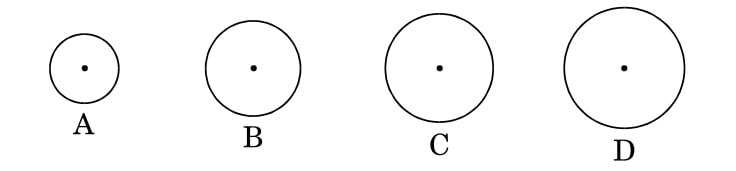
\includegraphics[width=\columnwidth]{cirls.png}
    \caption{Cirls}
    \label{fig:copper coins}
    \end{figure}
      
    \begin{itemize}
     \item   Fill in the diameters of the coins required in the following table :
    \begin{figure}[H]
        \centering
        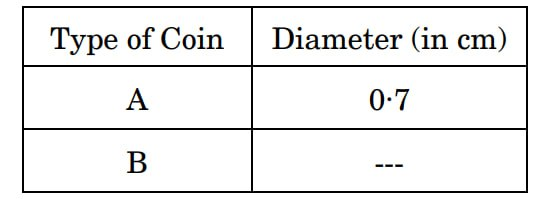
\includegraphics[width=\columnwidth]{table.png}
        \caption{table}
        \label{fig:enter-label}
    \end{figure}
    \item Complete the following table :
\begin{figure}[H]
    \centering
    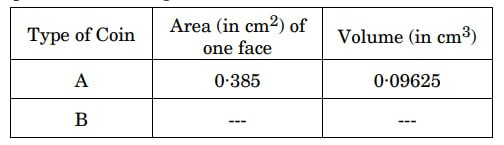
\includegraphics{2nd table.png}
    \caption{table}
    \label{fig:enter-label}
\end{figure}
\end{itemize}
\newpage
\item A well of diameter $3 m$ is dug $14 m$ deep. The earth 
       taken out of it has been spread evenly all around it in the shape of a circular ring of width
        $4 m$ to form a platform. Find the height of the platform. (Take $\pi=\frac{22}{7}$)

\item  A solid metallic sphere of radius $10.5 cm$ is melted and recast into a number of smaller cones, each of radius $3.5 cm$ and height $3 cm$. Find the number of cones so formed.

\item  In Figure 2, from a solid cube of side $7 cm$, a cylinder of radius $2.1 cm$ and height $7 cm$ is scooped out. Find the total surface area of the remaining solid.
\begin{figure}[H]
\centering
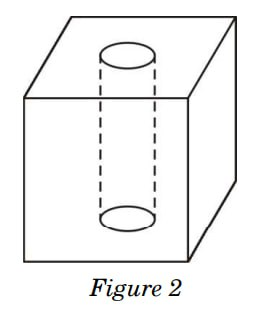
\includegraphics[width=0.4\columnwidth]{solid cube.png}
\caption{soild cube}
\label{fig:enter-label}
\end{figure}
\begin{center}
    OR
\end{center}
\item  A well of diameter $5 m$ is dug $24 m$ deep. The earth taken out of it has been spread evenly all around it in the shape of a circular ring of width $3 m$ to form an embankment. Find the height of the embankment.

 \item  A solid piece of metal in the form of a cuboid of dimensions $11 cm\times 7 cm\times 7 cm$ is melted to form n number of solid spheres of radii $\frac{7}{2}cm$ each. Find the value of $n$.
\newpage     
\item  A 'circus' is a company of performers who put on shows of acrobats, clowns etc. to entertain people started around $250$ years back, in open fields, now generally performed in tents
\\
One such 'Circus Tent' is shown below.
 \begin{figure}[H]
 \centering
 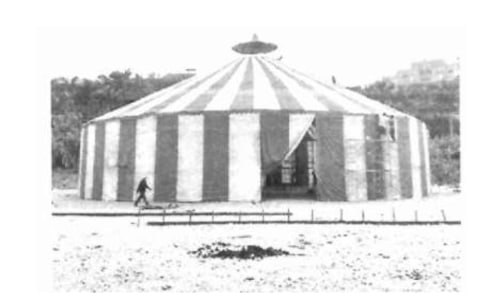
\includegraphics[width=\columnwidth]{circus tent.png}
 \caption{circus tent}
 \label{fig:circus tent.png}
 \end{figure}
  The tent is in the shape of a cylinder surmounted by a conical top. if the height and diameter of cylinder part are $9 m$ and $30 m$ respectively and height of conical part is 8 cm with same diameter as that of the cylindrical part, then find.
    \begin{enumerate}
    \item  The area of the canvas used in making the tent
    \item  The cost of the canvas bought for the tent at the rate \rupee~200 per sq. m, if 30 sq m canvas was wasted during stitching.
    \end{enumerate}
\newpage
\item 
\begin{enumerate}
   \item $150$ spherical marbles, each of diameter $1.4 cm$ are dropped in a cylinder vessel of diameter $7cm$ containing some water, and are completely immersed in water.Find the rise in the level of water in the cylindrical vessel
\begin{center}
       OR
\end{center}
\item Three cubes of side $6cm$ each,are joined as shown in Figure 2
\begin{figure}[H]
\centering
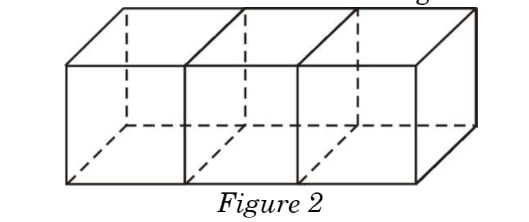
\includegraphics[width=0.6\columnwidth]{cuboid.png}
\caption{Cuboid}
\label{fig:cuboid}
\end{figure}
\end{enumerate}

\item In the picture given below, one can see a rectangular in-ground swimming pool installed by a family in their backyard. There is a concrete sidewalk around the pool of width $x m$. The outside edges of the sidewalk measure $7 m$ and $12 m$. The area of the pool is $36 sq. m$.
\begin{figure}[H]
    \centering
    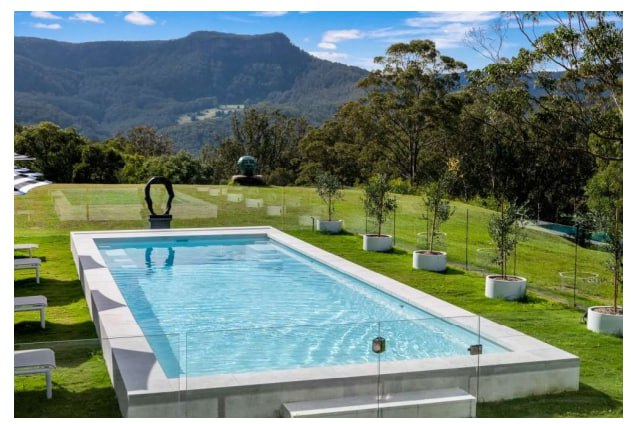
\includegraphics[width=\columnwidth]{swimming pool.png}
    \caption{swimming pool}
    \label{fig:swimming pool}
\end{figure}
\begin{enumerate}
    \item Based on the information given above, form a quadratic equation in terms of $x$
    \item Find the width of the sidewalk around the pool.
\end{enumerate}

\item John planned a birthday party for his younger sister with his friends. They decided to make some birthday caps by themselves and to buy a cake from a bakery shop. For these two items, they decided the following dimensions:
\\
Cake : Cylindrical shape with diameter $24 cm$ and height $14 cm.$

Cap : Conical shape with base circumference $44 cm$ and height $24 cm.$
\begin{figure}[H]
    \centering
    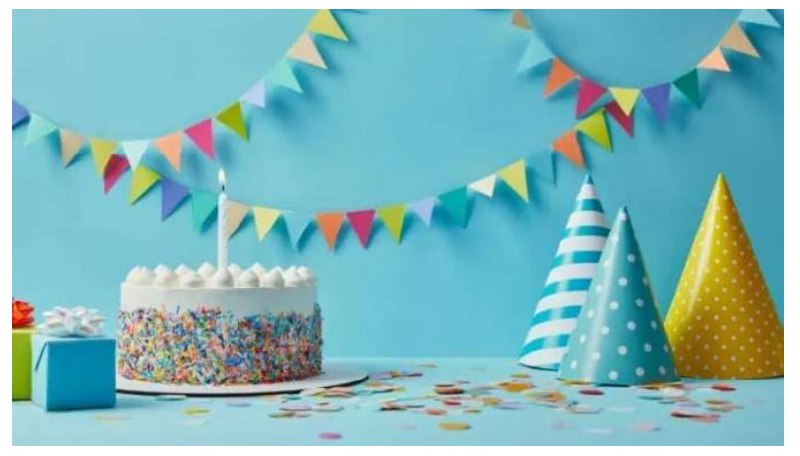
\includegraphics[width=\columnwidth]{birthday cake.png}
    \caption{birthday cake}
    \label{fig:birthday cake}
\end{figure}
Based on the above information, answer the following questions :
\begin{enumerate}
    \item How many square cm paper would be used to make 4 such caps ?
    \item The bakery shop sells cakes by weight $(0.5 kg, 1 kg, 1.5 kg, etc.).$ To have the required dimensions, how much cake should they order, if $650 cm^3$ equals $100 g$ of cake ?
\end{enumerate}
\newpage
\item 
\begin{enumerate}
    \item The curved surface area of a right circular cylinder is $176 sq cm$ and its volume is$1232 cu cm$ what is the height of the cylinder?
    \begin{center}
        OR
    \end{center}
    \item The largest sphere is carved out of a solid cube of side $21cm$ Find the volume of sphere
\end{enumerate}
\item Khurja is a city in the Indian state of Uttar Pradesh famous for the pottery.Khurja pottery is traditional Indian pottery work which has attracted Indians as well as foreighners with a variety of tea sets,crockery and ceramic tile works. A huge portion of the ceramics used in the country is supplied by Khurja and is also referred as 'The Ceramic Town'
One of the private schools of Bulandshahr organised an Educational Tour for class 10 students to Khurja. Students were very excited about the trip. Following are the few pottery objects of Khurja
\begin{figure}[H]
    \centering
    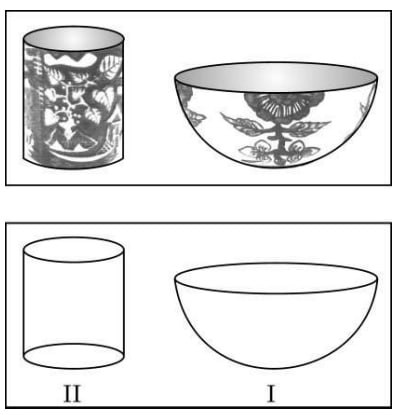
\includegraphics[width=0.4\columnwidth]{pottery.png}
    \caption{pottery}
    \label{fig:pottery}
\end{figure}
Students found the shapes of the objects very interesting and they could easily relate them with mathematical shapes viz sphere, hemisphere, cylinder etc. Maths teacher who was accompanying the students asked following question:
\begin{enumerate}
    \item The internal radius of hemispherical bowl(filled completely with water)in I is $9cm$ and radius and height of cylindrical jar in II is $1.5cm$ and $4cm$ respectively. If the hemisherical bowl is to be emptied in cylindrical jars, then how many cylindrical jars are required?
    \item If in the cylindrical jar full of water, a conical funnel of same height and same diameter is immersed, then how much water will flow out of the jar?
\end{enumerate}
\newpage
\item How many spherical shots each having diameter $3 cm$ can be made by melting a cuboidal solid of dimensions $18 cm\times 22 cm\times 6 cm$ ?
\item Conical bottom tanks in which an inverted cone at the bottom is surmounted by a cylinder of same diameter, are very advantageous in industry, specially where getting every last drop from the tank is important.

Vikas designed a conical bottom tank where the height of the conical part is equal to its radius and the height of the cylindrical part is two times of its radius. The tank is closed from the top.
\begin{enumerate}
    \item If the radius of the cylindrical part is $3 m$, then find the volume of the tank.
    \item Find the ratio of the volume of the cylindrical part to the volume of the conical part.
\end{enumerate}
              


    
\end{enumerate}

\end{document}

